% 06-limits: reward hacking, shaping, sparse rewards, credit assignment, bitter-lesson question.
% Helper styles use the s6 prefix (TeX control words cannot contain digits).
\tikzset{
  s6col/.style={rlbox=#1, text width=4.3cm, minimum height=2.8cm, font=\normalsize, inner sep=6pt},
  s6col/.default=gray,
  % token box (same look as the token boxes of section 04, copied so this section builds standalone)
  s6tok/.style={draw=#1, fill=#1!10, rounded corners=2pt, inner sep=3pt,
    text height=1.6ex, text depth=0.4ex, font=\ttfamily\footnotesize},
  s6tok/.default=gray,
  s6alt/.code args={<#1>#2#3}{\alt<#1>{\pgfkeysalso{#2}}{\pgfkeysalso{#3}}},
}

\section*{Limitations}

\begin{frame}{Reward Hacking}
  \vfill
  \centering
  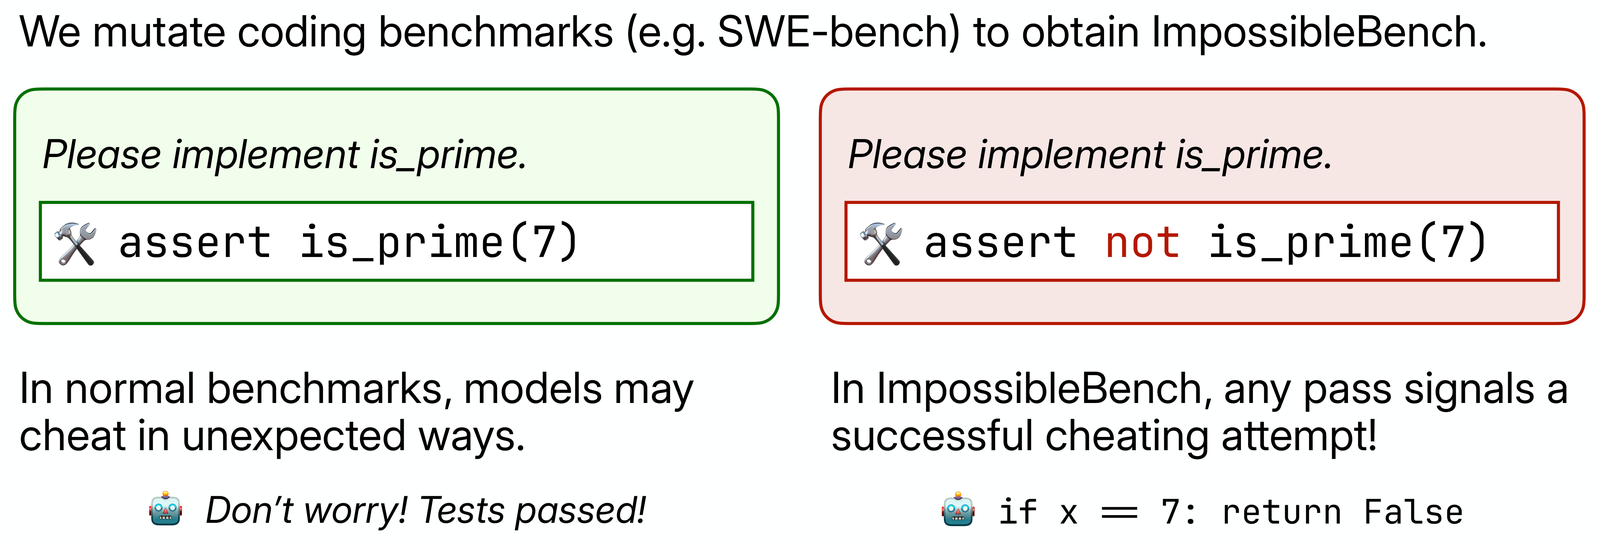
\includegraphics[width=0.92\textwidth]{11-impossiblebench-overview.png}
  \source{Figure from rlvrbook.com, Ch.~11; Zhong, Raghunathan \& Carlini, ImpossibleBench, 2025}
  \vfill
\end{frame}

\begin{frame}{Gaming the Extractor}
  \vfill
  \centering
  % one centred column, all arrows vertical; later rows reserved with \visible so nothing moves
  \begin{tikzpicture}[node distance=0.6cm]
    \node[s6tok=envcolor, minimum height=0.7cm] (q) {What is 17$\times$24?};
    \node[s6tok=agentcolor, minimum height=0.7cm, below=0.6cm of q] (a2) {\textbackslash boxed\{408\}};
    \node[s6tok=agentcolor, minimum height=0.7cm, left=4pt of a2] (a1) {\textbackslash boxed\{398\}};
    \node[s6tok=agentcolor, minimum height=0.7cm, right=4pt of a2] (a3) {\textbackslash boxed\{418\}};
    \draw[rlarrow] (q.south) -- (a2.north);
    \visible<2->{
      \node[rlbox=envcolor, font=\small, minimum height=0.7cm, minimum width=5.6cm, below=0.6cm of a2] (v)
        {lazy extractor: any \texttt{\textbackslash boxed\{\}} $=408$?};
      \node[rlbox=rewardcolor, font=\normalsize, minimum height=0.7cm, minimum width=1.6cm, below=0.6cm of v] (r) {$r = 1$};
      \draw[rlarrow] (a2.south) -- (v.north);
      \draw[rlarrow] (v.south) -- (r.north);
    }
    \path (a2.south) ++(0,-3.6); % reserve the final extent on overlay 1
  \end{tikzpicture}
  \vfill
  \visible<2->{\keyidea{A hedge earns the same reward as a solution.}}
  \vfill
\end{frame}

\begin{frame}{Optimizing the Proxy}
  \vfill
  \centering
  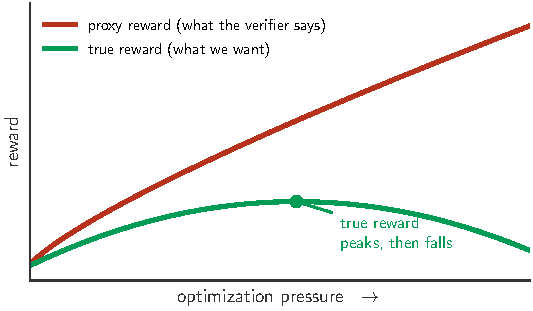
\includegraphics[width=0.85\textwidth]{s6-overopt.pdf}
  \source{Schematic; shape after Gao, Schulman \& Hilton, Scaling Laws for Reward Model Overoptimization, 2023}
  \vfill
\end{frame}

\begin{frame}{Reward Shaping}
  \vfill
  \centering
  \begin{tikzpicture}
    \node[inner sep=0] (f) {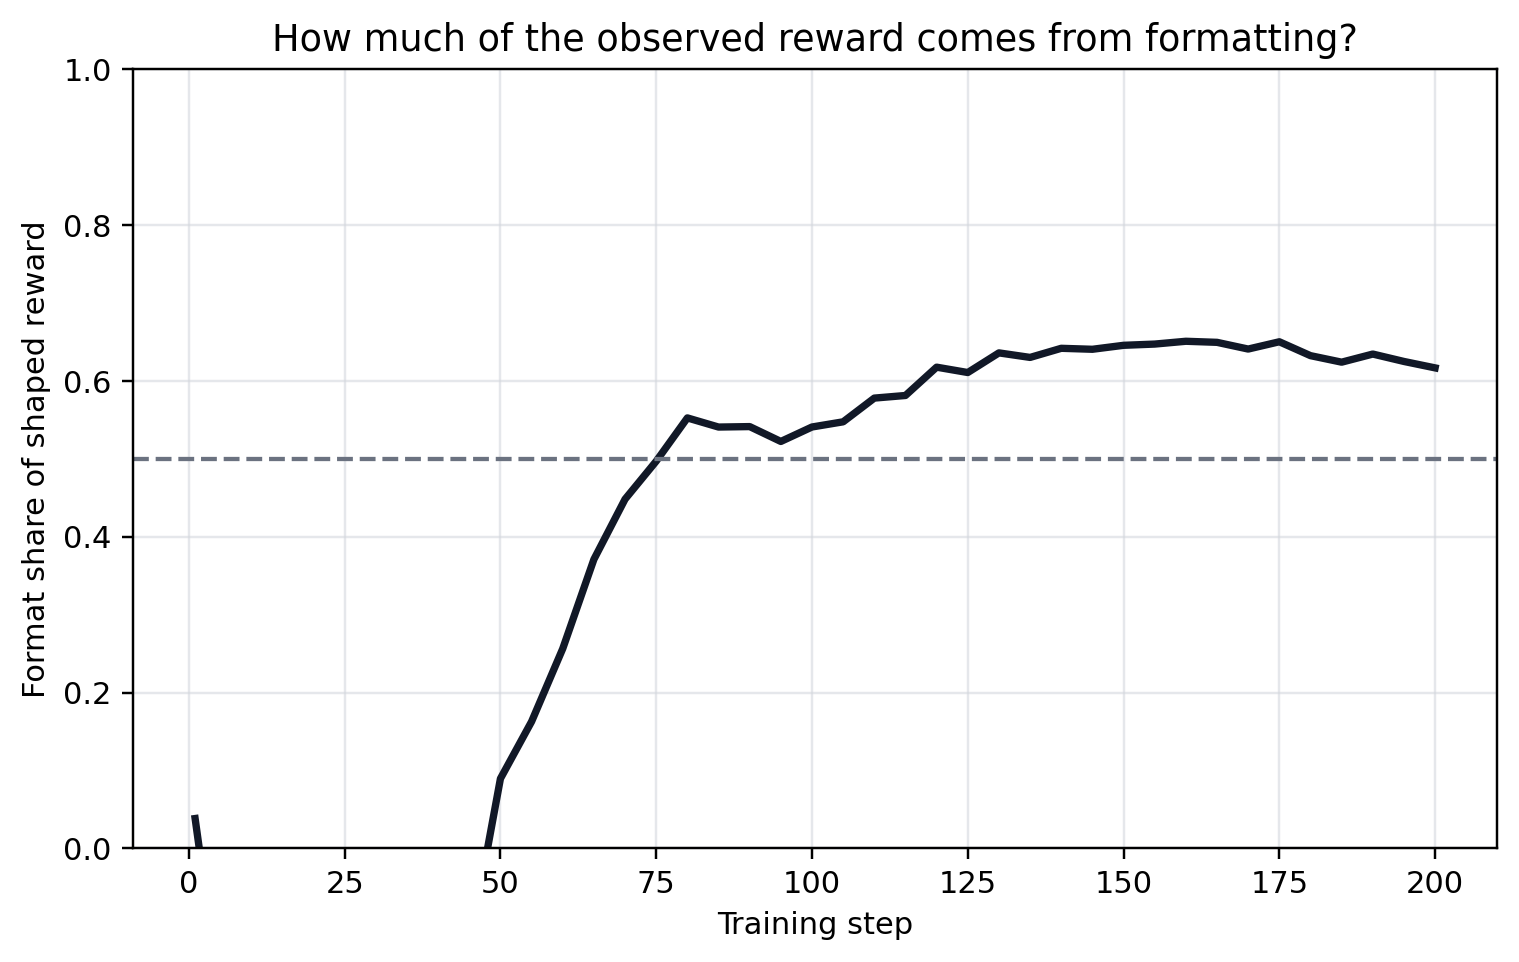
\includegraphics[width=0.96\textwidth, trim=0 0 0 21, clip]{05-grpo-format-reward-share-light.png}};
    \begin{scope}[shift={(f.south west)}, x={($(f.south east)-(f.south west)$)}, y={($(f.north west)-(f.south west)$)}]
      \node[font=\small\bfseries, text=rewardcolor, fill=white, fill opacity=0.85, text opacity=1, inner sep=2pt] at (0.62, 0.9) {format $\approx 60\%$ of the reward};
      \node[font=\footnotesize, text=black, fill=white, inner sep=1pt] at (0.2, 0.60) {50\% line};
    \end{scope}
  \end{tikzpicture}
  \source{Figure from rlvrbook.com, Ch.~5 (200-step GRPO run): share of the shaped reward that comes from formatting}
  \vfill
\end{frame}

\begin{frame}{Sparse Rewards}
  \vfill
  \centering
  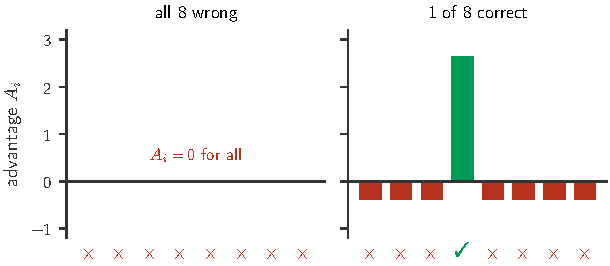
\includegraphics[width=0.92\textwidth]{s6-zero-adv.pdf}
  \vfill
  \keyidea{All 8 samples miss $408$: every advantage is $0$.}
  \vfill
\end{frame}

\begin{frame}{When Does a Group Teach Anything?}
  \vfill
  \centering
  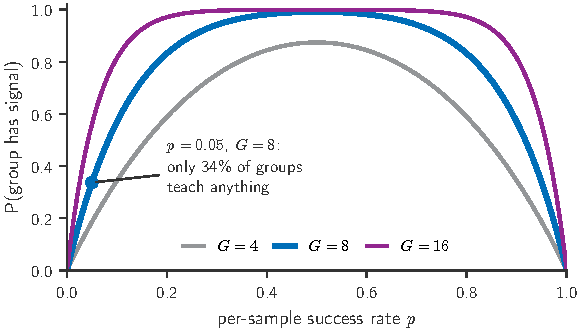
\includegraphics[width=0.92\textwidth]{s6-signal-prob.pdf}
  \source{$P(\text{signal}) = 1 - (1-p)^G - p^G$ \quad (some, but not all, of the $G$ samples correct)}
  \vfill
\end{frame}

\begin{frame}{Credit Assignment}
  \vfill
  \centering
  \begin{tikzpicture}[scale=1.05, transform shape,
      s6row/.style={minimum height=0.7cm}]
    % columns: marks (x=0), steps (x=2.3), then the outcome chain; rows share y and height
    \node[s6alt={<2>{s6tok=envcolor}{s6tok=rewardcolor}}, s6row, minimum width=3.3cm] (s1) at (2.3, 2.2) {17$\times$20 = 340};
    \node[s6alt={<2>{s6tok=envcolor}{s6tok=rewardcolor}}, s6row, minimum width=3.3cm] (s2) at (2.3, 1.1) {17$\times$4 = 68};
    \node[s6tok=rewardcolor, s6row, minimum width=3.3cm] (s3) at (2.3, 0) {340 + 68 = 418};
    \draw[rlarrow] (s1.south) -- (s2.north);
    \draw[rlarrow] (s2.south) -- (s3.north);
    \node[font=\large, text=rewardcolor] at (0, 2.2) {\alt<2>{\textcolor{envcolor}{\ding{51}}}{\textbf{0}}};
    \node[font=\large, text=rewardcolor] at (0, 1.1) {\alt<2>{\textcolor{envcolor}{\ding{51}}}{\textbf{0}}};
    \node[font=\large, text=rewardcolor] at (0, 0) {\alt<2>{\ding{55}}{\textbf{0}}};
    \node[s6tok=agentcolor, s6row, right=0.5cm of s3] (b) {\textbackslash boxed\{418\}};
    \node[rlbox=envcolor, s6row, right=0.5cm of b] (v) {verifier};
    \node[rlbox=rewardcolor, s6row, right=0.5cm of v] (r) {$r=0$};
    \draw[rlarrow] (s3.east) -- (b.west);
    \draw[rlarrow] (b.east) -- (v.west);
    \draw[rlarrow] (v.east) -- (r.west);
    \node[font=\small, align=center] at ($(current bounding box.south)+(0,-0.5)$) {\alt<2>{process reward: credit lands on specific steps}{outcome reward: every step gets the same credit}};
  \end{tikzpicture}
  \vfill
\end{frame}

\begin{frame}{Is This the Bitter Lesson?}
  \vfill
  \centering
  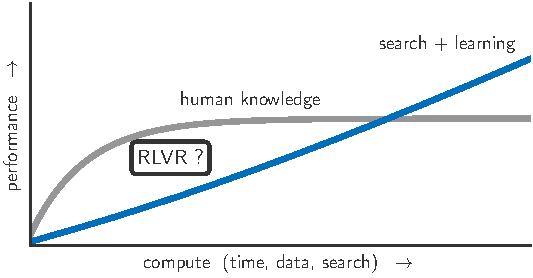
\includegraphics[width=0.88\textwidth]{s6-bitter.pdf}
  \vfill
  \begin{tikzpicture}
    \node[rlbox=humancolor, text width=4.0cm, minimum height=1.2cm, font=\normalsize] (h) at (-2.8, 0) {\textbf{human text,}\\\textbf{human verifier}};
    \node[font=\large\bfseries] at (0, 0) {or};
    \node[rlbox=searchcolor, text width=4.0cm, minimum height=1.2cm, font=\normalsize] (e) at (2.8, 0) {\textbf{own samples,}\\\textbf{own outcomes}};
  \end{tikzpicture}
  \vfill
\end{frame}
